\documentclass[12pt]{article}
\usepackage{rocca-homework}
\usepackage{graphicx}

\begin{document}

\title{CS 350 Homework 1}
\author{Lucas Vas}

\maketitle

\section*{Problem 1}

The class diagram that I came up with for the book is something like this:

\begin{center}
	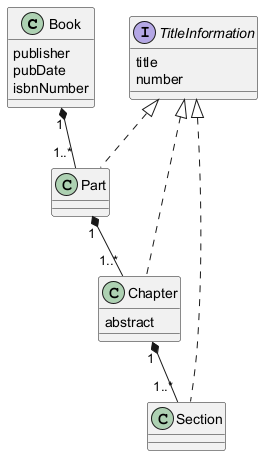
\includegraphics[height=4in]{BookClassDiagram}
\end{center}

\clearpage
The object diagram would then look a little like this:

\begin{center}
	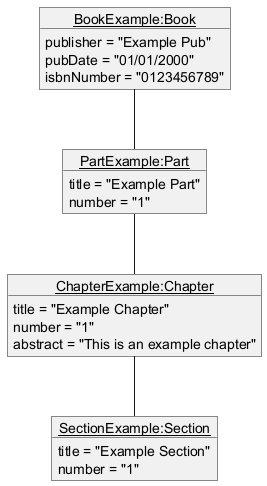
\includegraphics[height=4in]{BookObjectDiagram}
\end{center}

\clearpage
\section*{Problem 2}

The activity diagram for a pizza order would looks like this:

\begin{center}
	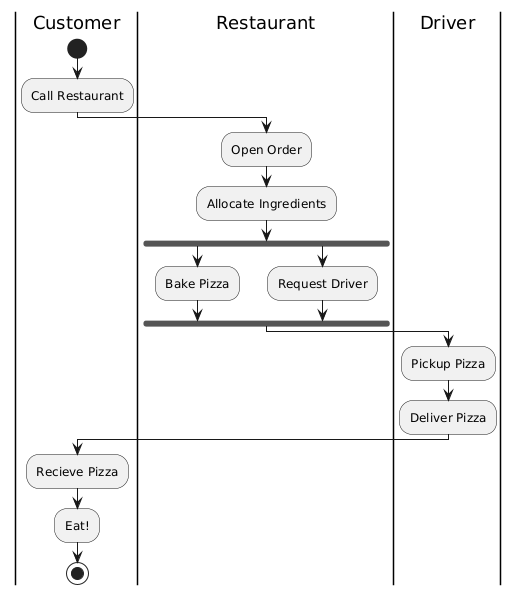
\includegraphics[height=4in]{pizzaUMLNoErrors}
\end{center}

\clearpage
And then we add the fact that we can have errors:

\begin{center}
	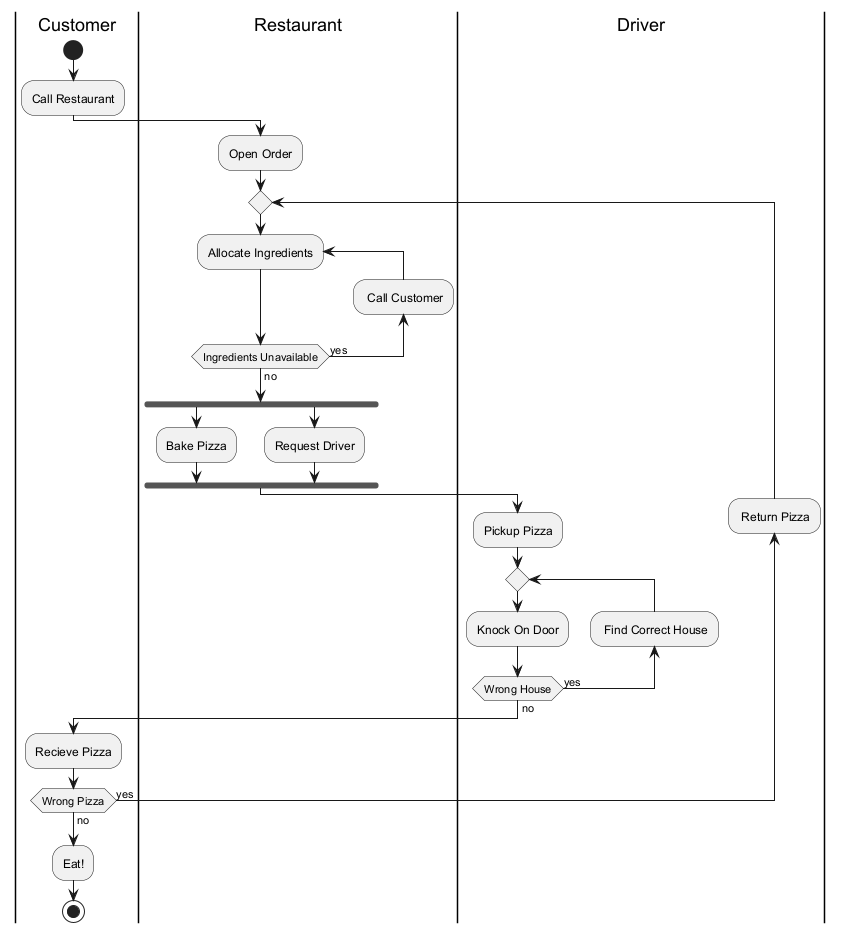
\includegraphics[height=6in]{pizzaUMLWithErrors}
\end{center}

\clearpage
\section*{Problem 3}

Our Debian-based server update process would look like this in a sequence diagram:

\begin{center}
	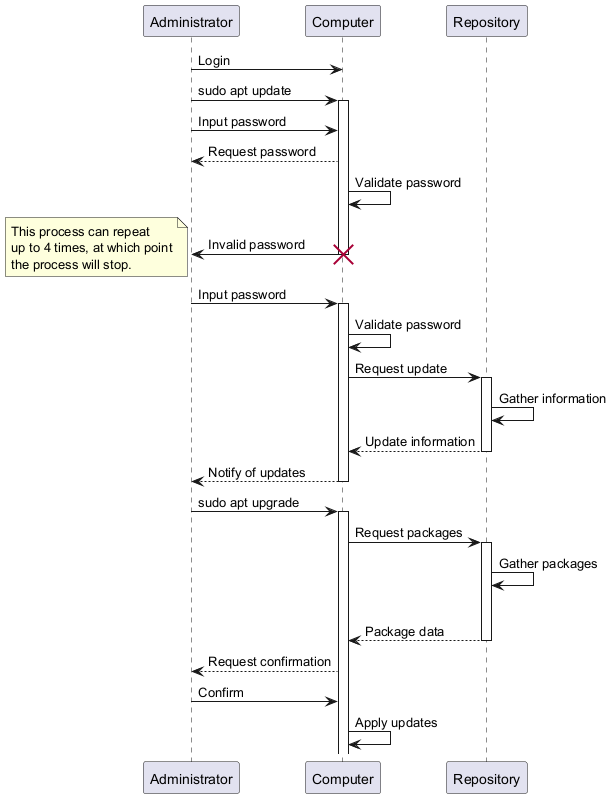
\includegraphics[height=6in]{DebianServerUpdateDiagram}
\end{center}

\end{document}
